\section*{Part 3 [68 points]}

\begin{enumerate}

    % PART 1
    \item \textbf{[34 points]} Describe and analyze your hand-crafted policy. 
    \begin{enumerate}



    % QUESTION b
    \item \textbf{[17 points]} With your scheduling policy, run the entire workflow \textbf{\textcolor{red}{3 separate times}}. For each run, measure the execution time of each batch job, as well as the latency outputs of memcached, running with a steady client load of 30K QPS. For each batch application, compute the mean and standard deviation of the execution time \footnote{Here, you should only consider the runtime, excluding time spans during which the container is paused.} across three runs. Also, compute the mean and standard deviation of the total time to complete all jobs - the makespan of all jobs. Fill in the table below. Finally, compute the SLO violation ratio for memcached for the three runs; the number of data points with 95th percentile latency $>$ 1ms, as a fraction of the total number of data points. The SLO violation ratio should be calculated during the time from when the first batch-job-container starts running to when the last batch-job-container stops running.  \\

    \begin{table}[ht]
        \centering
        \begin{tabular}{ |c|c|c|} 
            \hline
            job name & mean time [s] & std [s] \\ \hline \hline
            \coloredcell{barnes}          & 63.33 & 1.53 \\  \hline
            \coloredcell{blackscholes}    & 47.67 & 3.06 \\  \hline
            \coloredcell{canneal}         & 107.33 & 1.53 \\  \hline
            \coloredcell{freqmine}        & 67.33 & 0.58 \\  \hline
            \coloredcell{radix}           & 20.67 & 2.08 \\  \hline
            \coloredcell{streamcluster}   & 113.33 & 16.20 \\  \hline
            \coloredcell{vips}            & 21.33 & 1.53 \\  \hline
            total time      & 232.33 & 3.06 \\  \hline
        \end{tabular}
    \end{table}

    \textbf{Answer:} The values in the table are computed from the container \texttt{startedAt} and \texttt{finishedAt} timestamps in \texttt{results.json}. In the augmented \texttt{mcperf} output, \texttt{ts\_start} and \texttt{ts\_end} are Unix epoch timestamps in milliseconds that bound the measurement interval represented by one p95 latency row. All three executions completed the seven batch jobs successfully. During the interval from the first batch container start to the last batch container finish, no measured memcached p95 sample exceeded the \(1\,\mathrm{ms}\) SLO; the resulting SLO violation ratio is \(0.000\).
    \\
    
    Create 3 bar plots (one for each run) of memcached p95 latency (y-axis) over time (x-axis), with annotations showing when each batch job started and ended, also indicating the machine each of them is running on. Using the augmented version of mcperf, you get two additional columns in the output: \texttt{ts\_start} and \texttt{ts\_end}. Use them to determine the width of each bar in the bar plot, while the height should represent the p95 latency. Align the $x$ axis so that $x=0$ coincides with the starting time of the first container. 
    For each core in each machine show what job it is running using the colors proposed in this template (you can find them in \texttt{main.tex}). For example, draw a bar in {\color{vips}the color of vips} for core x from when vips is started to when it ends if vips ran on core x.
    %Use  the colors proposed in this template (you can find them in \texttt{main.tex}). For example, use the \colored{vips} color to annotate when vips started and stopped, the \colored{blackscholes} color to annotate when blackscholes started and stopped etc.

    \textbf{Plots:}

    \begin{figure}[H]
        \centering
        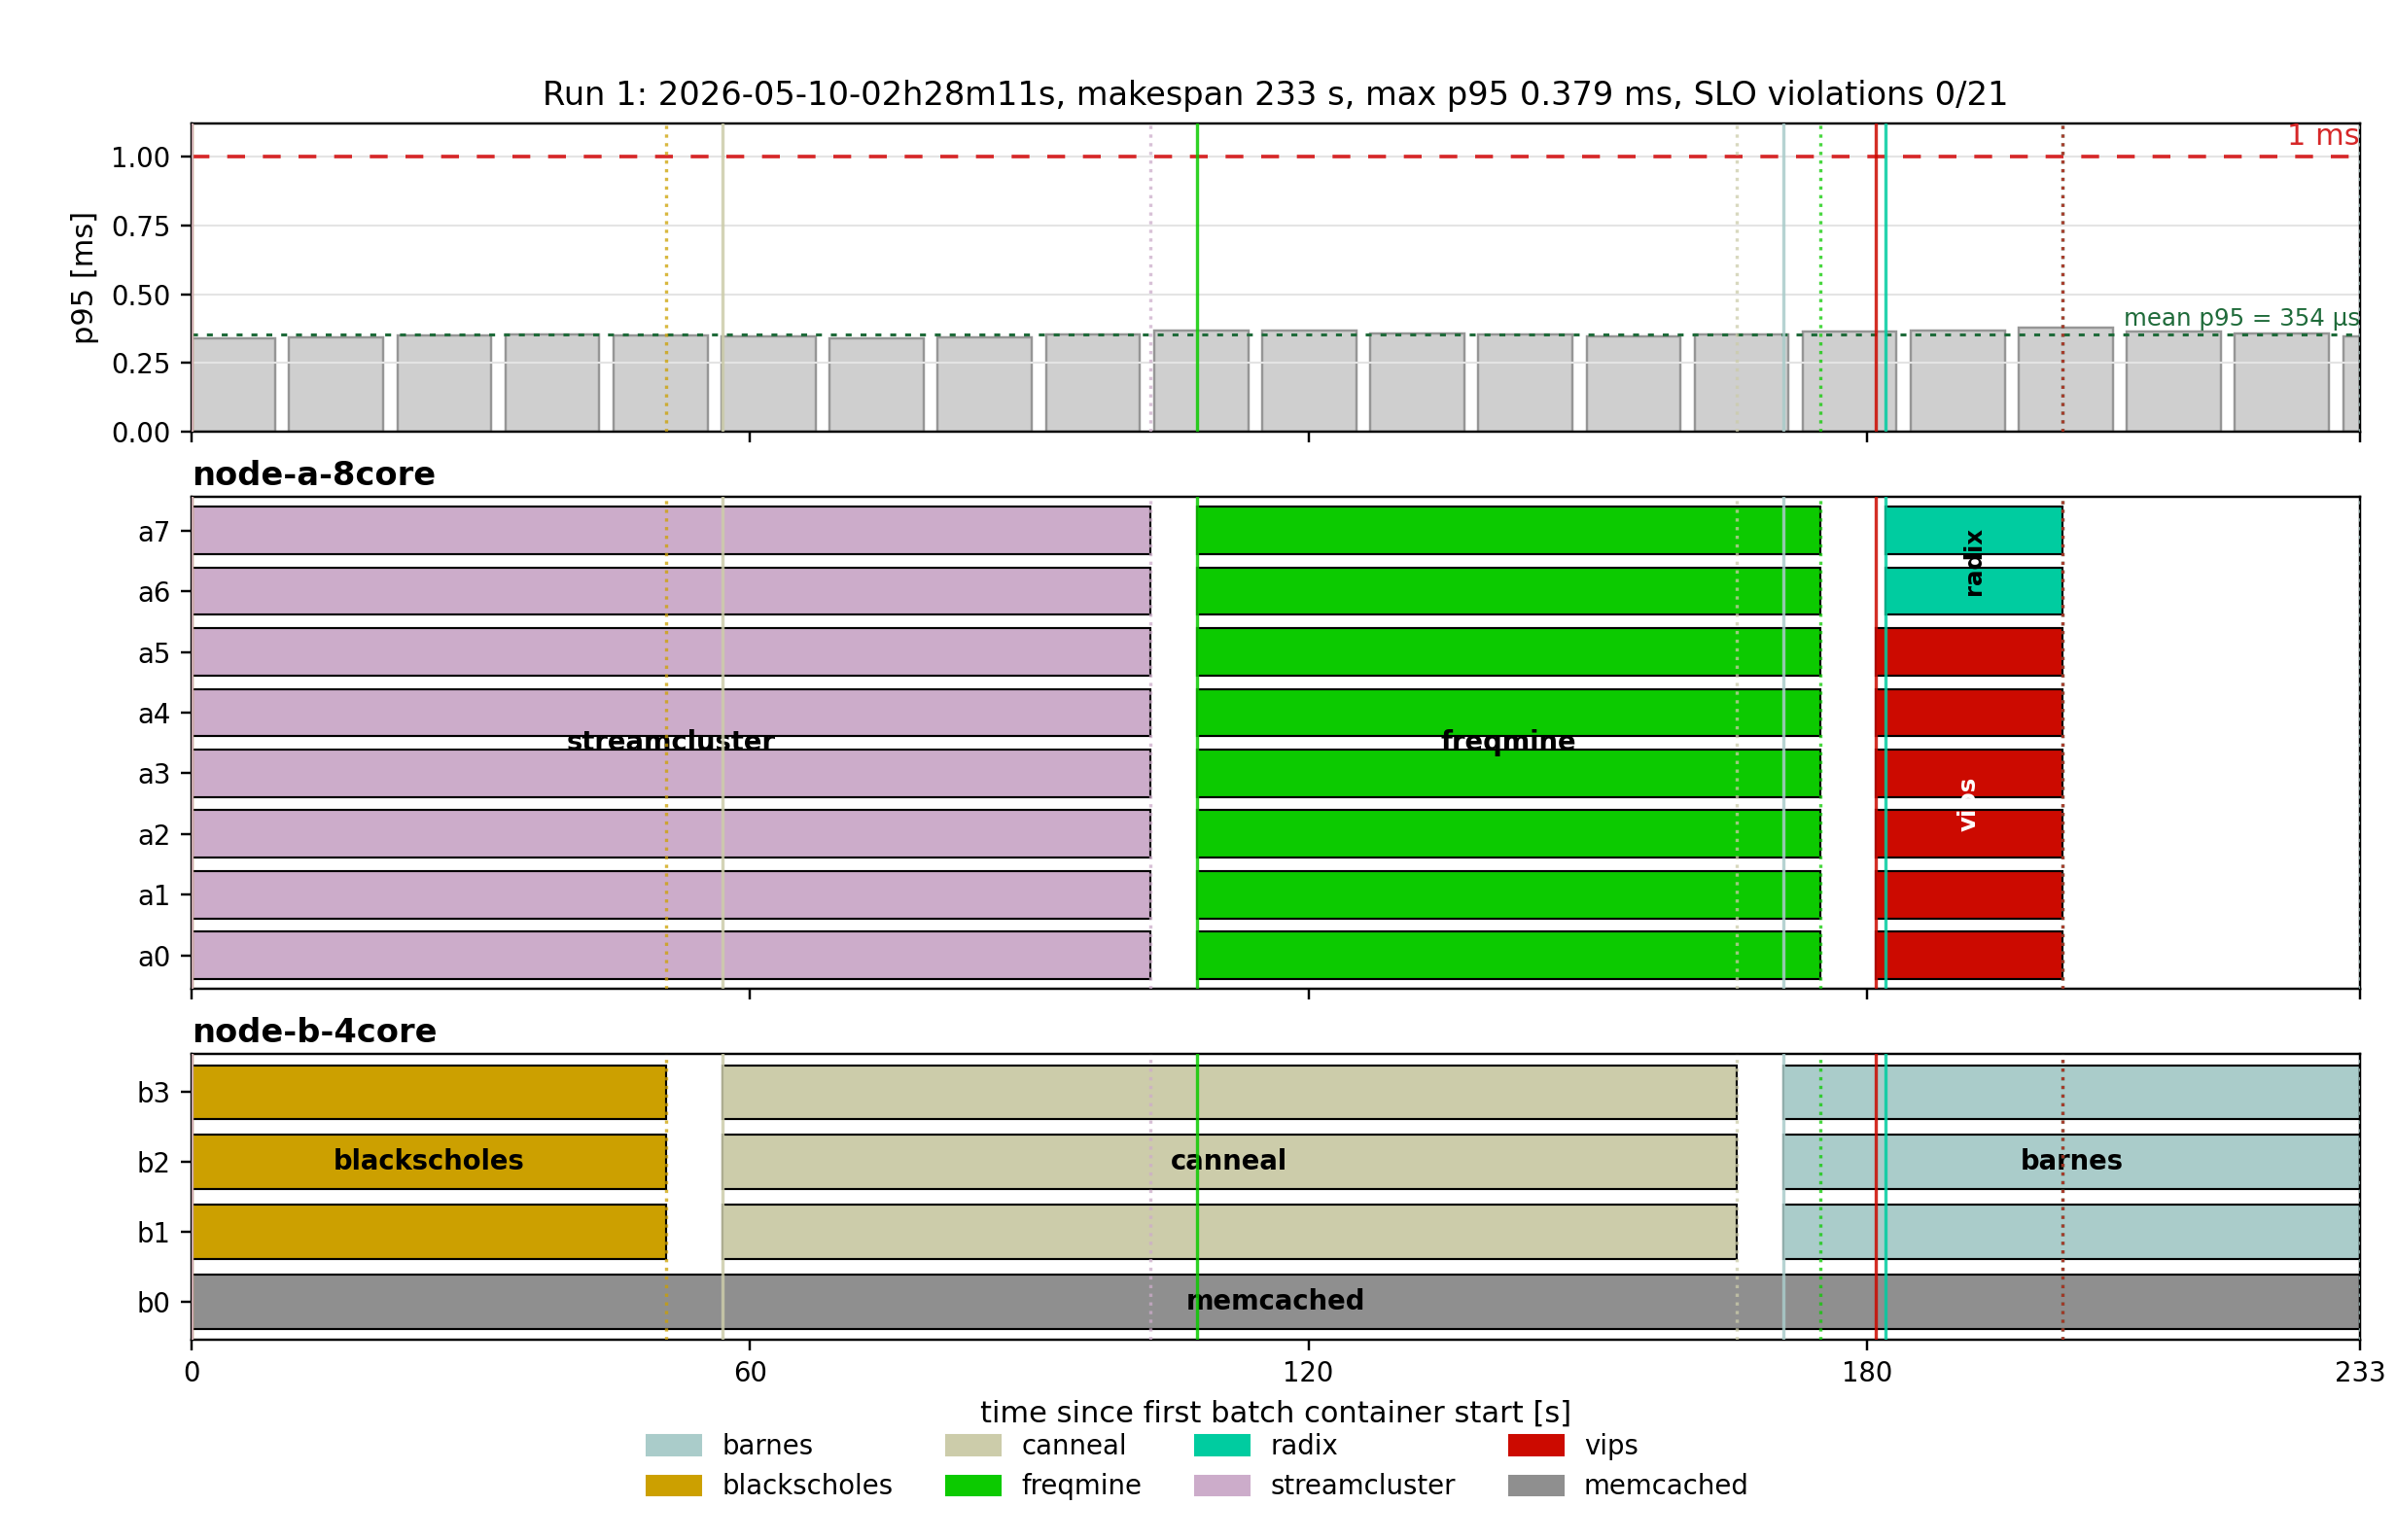
\includegraphics[width=\linewidth]{figures/cx_part3_q1a_run1.png}
        {\small Run~1 (\texttt{2026-05-10-02h28m11s}). Memcached p95 latency over time and per-core placement on \texttt{node-a-8core} and \texttt{node-b-4core}. The red dashed line marks the \(1\,\mathrm{ms}\) SLO.}
    \end{figure}

    \begin{figure}[H]
        \centering
        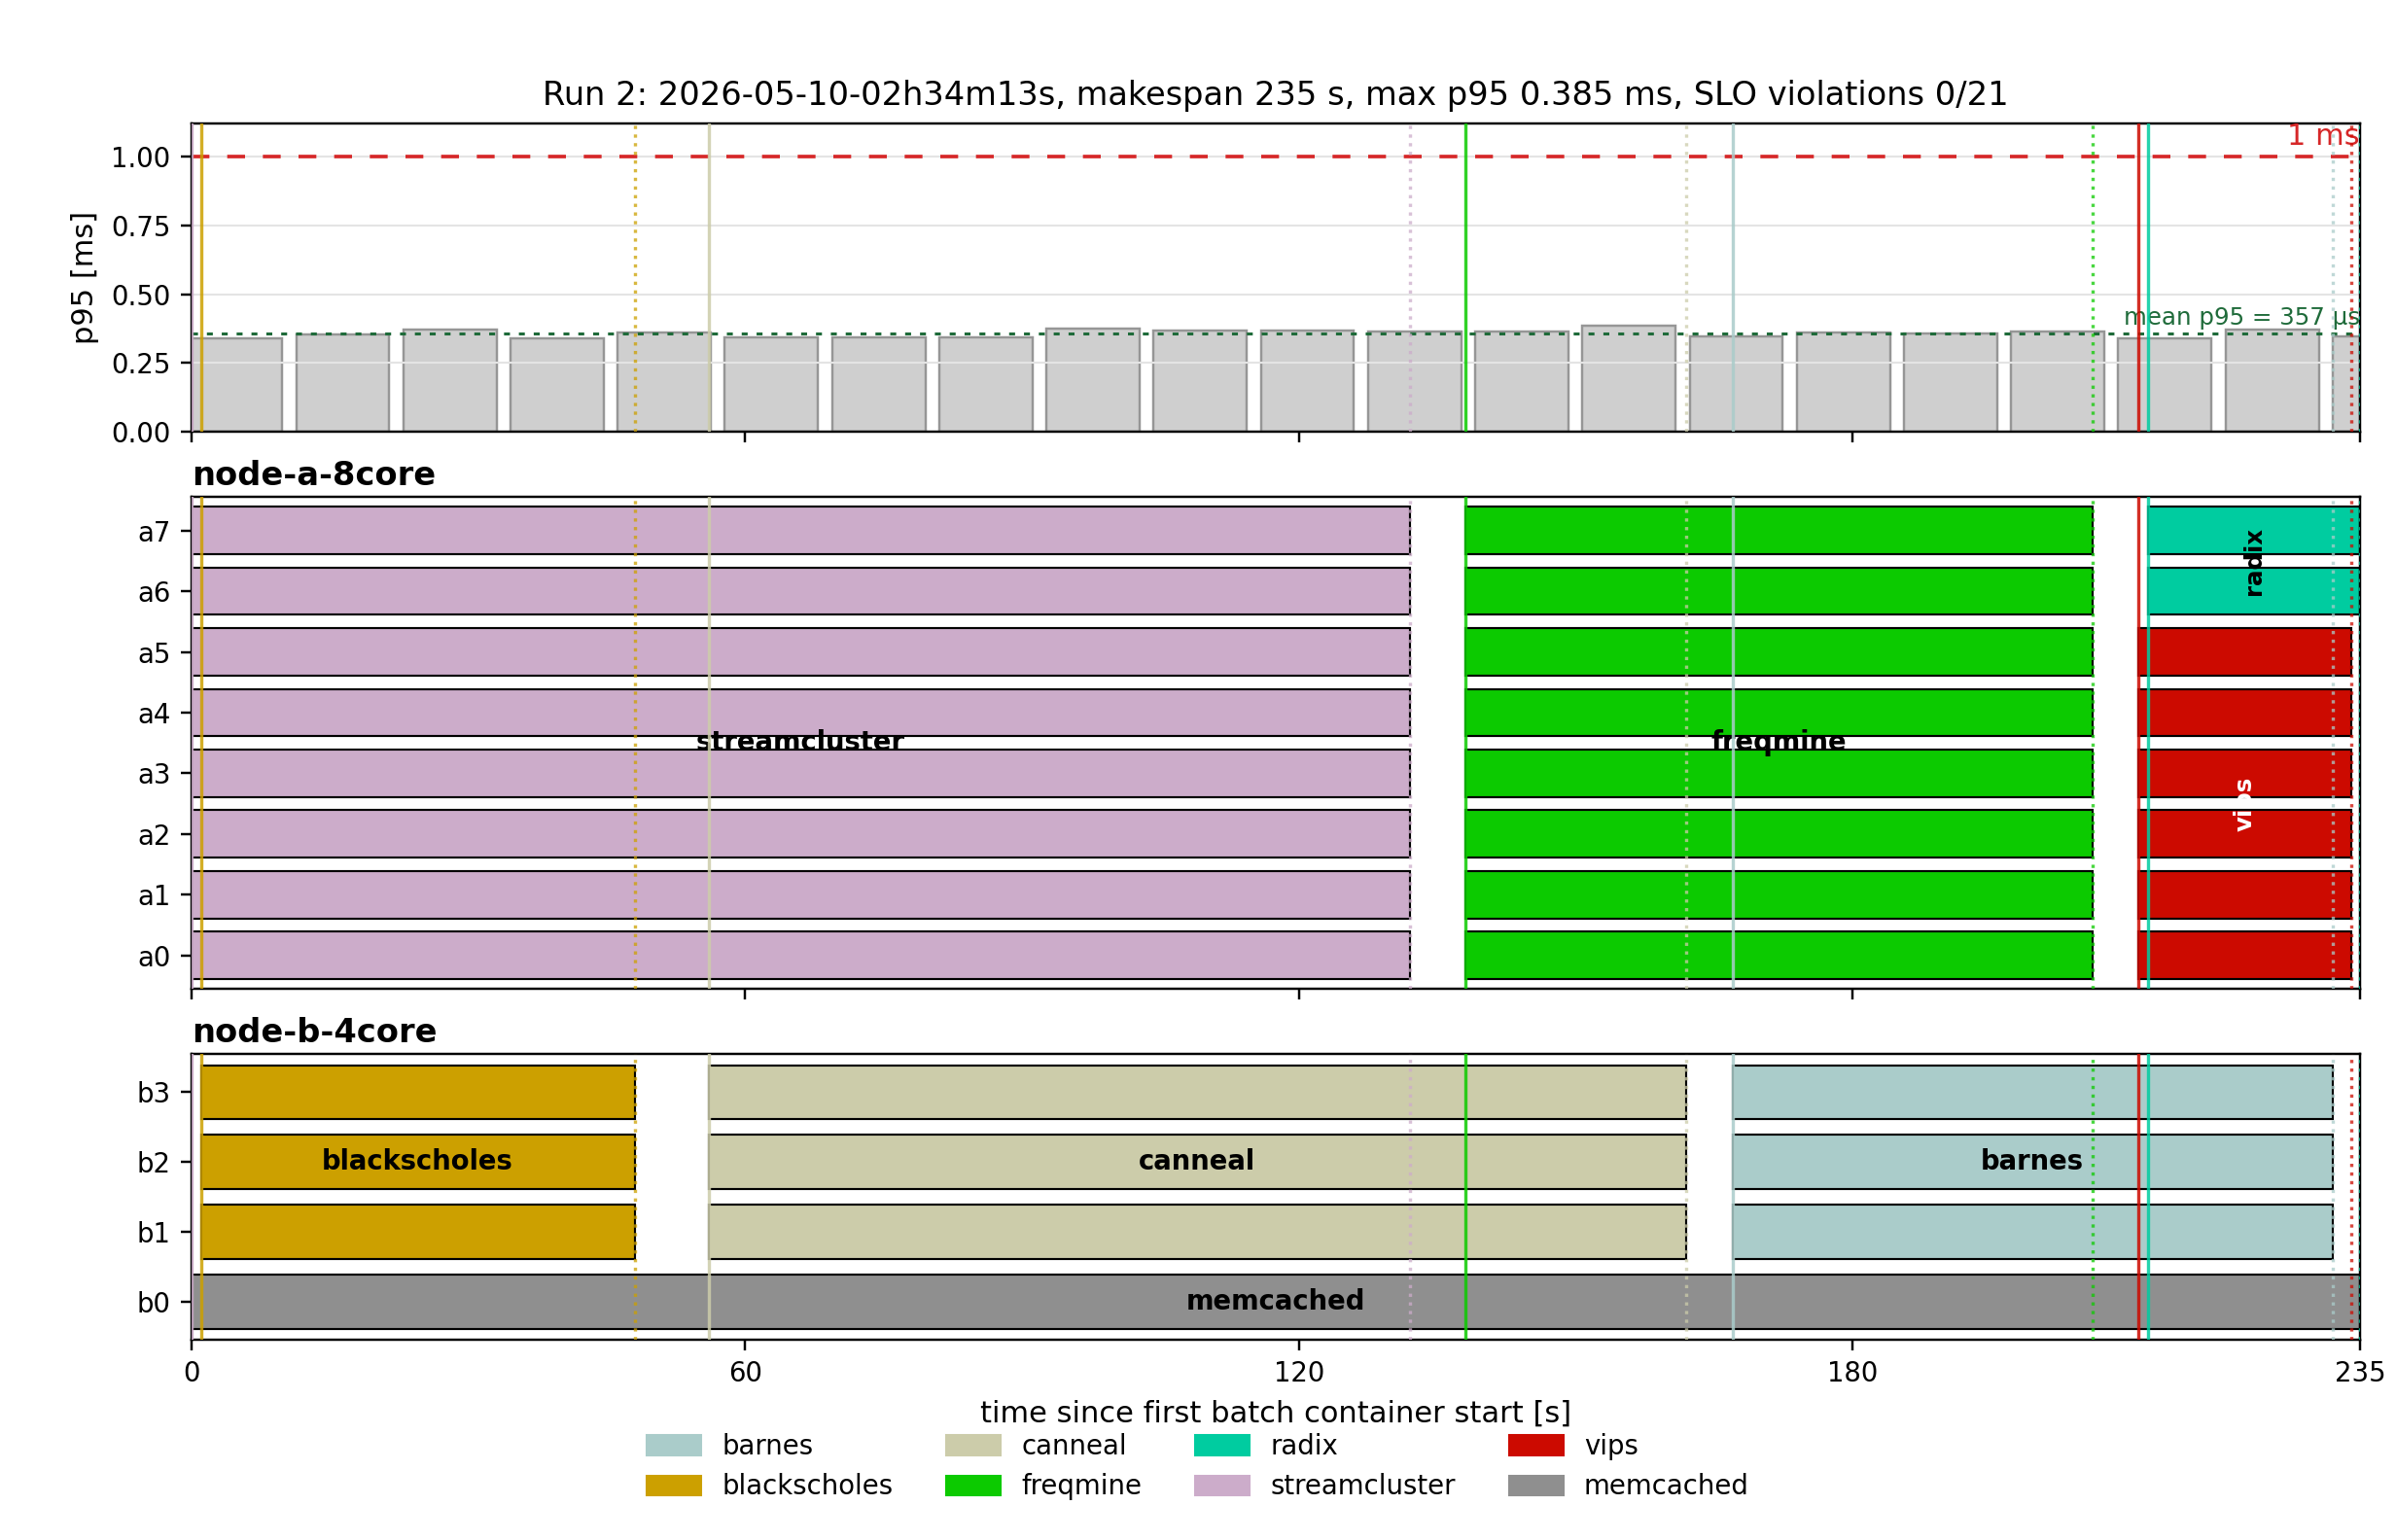
\includegraphics[width=\linewidth]{figures/cx_part3_q1a_run2.png}
        {\small Run~2 (\texttt{2026-05-10-02h34m13s}). Memcached p95 latency over time and per-core placement on \texttt{node-a-8core} and \texttt{node-b-4core}. The red dashed line marks the \(1\,\mathrm{ms}\) SLO.}
    \end{figure}

    \begin{figure}[H]
        \centering
        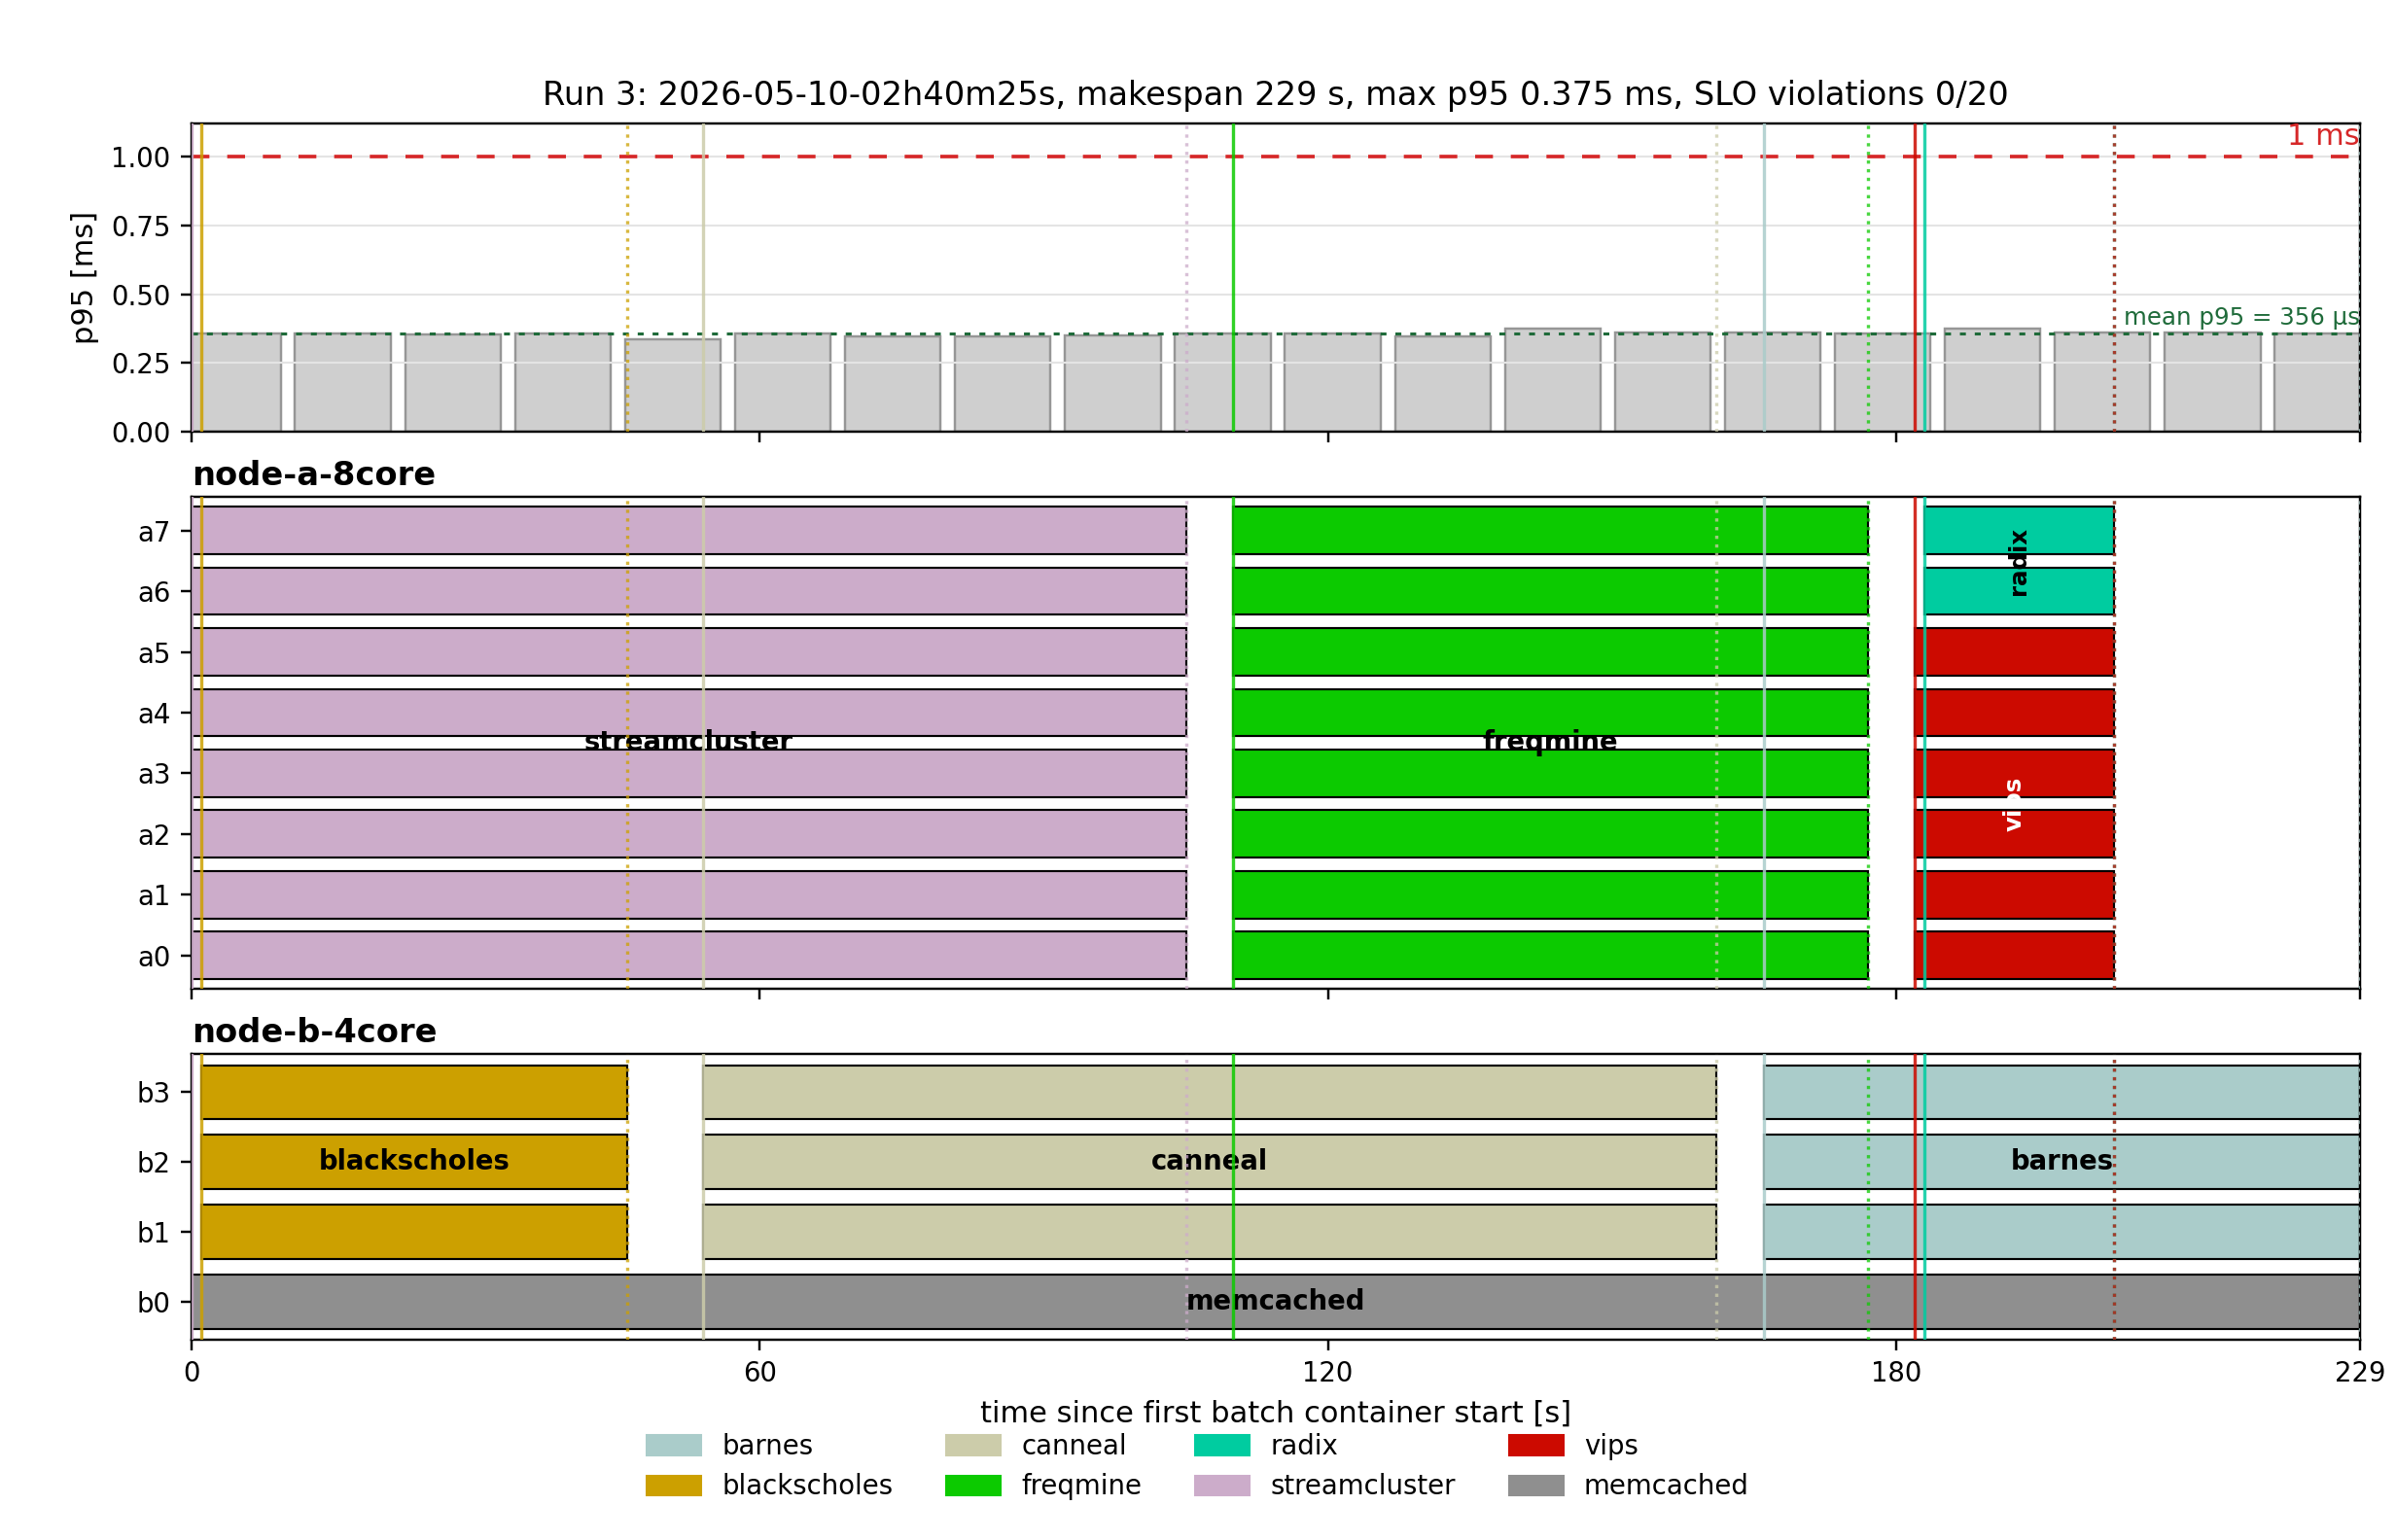
\includegraphics[width=\linewidth]{figures/cx_part3_q1a_run3.png}
        {\small Run~3 (\texttt{2026-05-10-02h40m25s}). Memcached p95 latency over time and per-core placement on \texttt{node-a-8core} and \texttt{node-b-4core}. The red dashed line marks the \(1\,\mathrm{ms}\) SLO.}
    \end{figure}
    % QUESTION b
    \item \textbf{[17 points]} Describe and justify the “optimal” scheduling policy you have designed. 
    
    \begin{itemize}
        \item Which node does memcached run on? Why?

        \textbf{Answer:} % Place your solution here.
        \\

        \item Which node does each of the 7 batch jobs run on? Why?

        \textbf{Answer:}
        \begin{itemize}
            \item \colored{barnes}: % Place your solution here .
            
            \item \colored{blackscholes}: % Place your solution here.
            
            \item \colored{canneal}: % Place your solution here.
            
            \item \colored{freqmine}: % Place your solution here.
            
            \item \colored{radix}: % Place your solution here.
            
            \item \colored{streamcluster}: % Place your solution here.
            
            \item \colored{vips}: % Place your solution here.
            \\
            
        \end{itemize}

        \item Which jobs run concurrently / are colocated? Why?

        \textbf{Answer:} % Place your solution here.
        \\

        \item In which order did you run the 7 batch jobs? Why?
    
        \textbf{Order (to be sorted)}: % Sort them 
        \colored{barnes}, \colored{blackscholes}, \colored{canneal}, \colored{freqmine}, \colored{radix}, \colored{streamcluster}, \colored{vips}
    
    
        \textbf{Why}: % Place your solution here.
        \\

        \item How many threads have you used for each of the 7 batch jobs? Why?
    
        \textbf{Answer:}
    
        \begin{itemize}
            \item \colored{barnes}: % Place your solution here. 
            
            \item \colored{blackscholes}: % Place your solution here.
            
            \item \colored{canneal}: % Place your solution here.
            
            \item \colored{freqmine}: % Place your solution here.
            
            \item \colored{radix}: % Place your solution here.
           
            \item \colored{streamcluster}: % Place your solution here.
            
            \item \colored{vips}: % Place your solution here.
            \\
        \end{itemize}

        \item Which files did you modify or add and in what way? Which Kubernetes features did you use?
    
        \textbf{Answer:} % Place your solution here.
        \\
    
        \item Describe the design choices, ideas and trade-offs you took into account while creating your scheduler (\underline{if not already mentioned above}). Describe how your policy (and its performance) compares to another policy that you experimented with (in particular to the second-best policy that you designed).

        \textbf{Answer:} % Place your solution here
        \\
    

    \end{itemize}
    \end{enumerate}


    % PART 2
    \item \textbf{[34 points]} Describe and analyze the AI-generated policy. [TODO: Xiaozhe]

    \begin{enumerate}

        % QUESTION a
        \item \textbf{[17 points]} \textbf{Report the performance}:
        
        \begin{itemize}
            \item Report the mean time of each batch job, as well as the makespan of all jobs for the AI-generated policy. Also, report the SLO violation ratio for memcached for the AI-generated policy. \textit{Note: If the LLM failed to produce a valid solution after 3+ attempts, provide the error logs and your best-performing manual tweak for partial credit.}
        
        \begin{table}[ht]
            \centering
            \begin{tabular}{ |c|c|c|c|c|} 
                \hline
                job name & mean time [s] (Baseline) & mean time [s] (AI) \\ \hline \hline
                \coloredcell{barnes}          & & \\  \hline
                \coloredcell{blackscholes}    & & \\  \hline
                \coloredcell{canneal}         & & \\  \hline
                \coloredcell{freqmine}        & & \\  \hline
                \coloredcell{radix}           & & \\  \hline
                \coloredcell{streamcluster}   & & \\  \hline
                \coloredcell{vips}            & & \\  \hline
                total time      & & \\  \hline
            \end{tabular}
        \end{table}

    \item Create 3 bar plots (one for each run), for the final AI-generated policy, of memcached p95 latency (y-axis) over time (x-axis), with annotations showing when each batch job started and ended, also indicating the machine each of them is running on. Use the same method as described in the previous question to create the bar plots.
    
    \textbf{Answer:}
    \item Create two line plots (one for the p95 latency and one for SLO violations) showing policy performance over iterations.
    
    \textbf{Answer:}
    \end{itemize}

    % QUESTION b
    \item \textbf{[17 points]} Analysis of the Evolutionary Process: Describe the process of how you used OpenEvolve to design the AI-generated policy. For example, you can include the following details in your answer (You are not limited to these questions. You can include any other details you find relevant and interesting). Your response will be graded based on the thoroughness of the exploration and clarity in explanation:
        
        \begin{itemize}
            \item How many iterations did you run through OpenEvolve with the LLMs to get to the final policy? Which LLM(s) did you use?
            \item How do you measure success? For example, how do you design the `combined\_score' or the success metric, given that there are two objectives (makespan and SLO violations)?
            \item Describe the initial policy you fed to the LLM(s) and why you chose this as the initial policy.
            \item Describe how the policy changes during the process, and how it impacted the performance of the policy (e.g., tail latency; SLO violations).
            \item Explain why did this AI-generated policy perform better (or worse) than the baseline?
            \item Identify one ``hallucination'' or logical flaw the model produced during the process and how you identified it.
        \end{itemize}

         \textbf{Answer:}


    \end{enumerate}

    Please attach your modified/added YAML files, run scripts, OpenEvolve scripts, experiment outputs and the report as a zip file. You can find more detailed instructions about the submission in the project description file.
    
    \textbf{Important: The search space of all possible policies is exponential and you do not have enough credits to run all of them. We do not ask you to find the policy that minimizes
    the total running time, but rather to design a policy that has a reasonable running time, does not violate the SLO, and takes into account the characteristics of the first two parts of the project.}
\end{enumerate}

\newpage
